%%%%%%%%%%%%%%%%%%%%%%%%%%%%%%%%%%%%%%%%%%%%%%%%%%%%%%%%%%%%%%%%%%%%%%%%%%%%%%%%%
\subsection{High-Order Scheme}
%%%%%%%%%%%%%%%%%%%%%%%%%%%%%%%%%%%%%%%%%%%%%%%%%%%%%%%%%%%%%%%%%%%%%%%%%%%%%%%%%
\begin{frame}
\frametitle{Introduction to Entropy Viscosity}

\begin{itemize}
   \item The standard Galerkin CFEM method does not necessarily produce the
      correct weak solution and may even diverge. Even with
      FCT, it would not necessarily converge to the correct, physical
      weak solution, i.e., the \emph{entropy} solution.
   \item To converge to the entropy solution, one must ensure that an entropy
      inequality is satisfied:
      \begin{equation}
         R(u) \equiv \pd{\eta(u)}{t} + \nabla\cdot\mathbf{f}^\eta(u) \leq 0
      \end{equation}
      for any convex entropy $\eta(u)$ and corresponding entropy flux
      $\mathbf{f}^\eta(u)$.
   %\item Note that the entropy inequality in mathematics is flipped from
   %   its definition in thermodynamics, where entropy is a non-\emph{decreasing}
   %   function.
   \item This \emph{entropy residual} $R(u)$ measures entropy production;
      where it is positive, the inequality is violated, so the residual
      should be decreased somehow.
   \item To enforce the inequality, the entropy viscosity method adds
      viscosity in proportion to local entropy production, thus decreasing
      local entropy.
\end{itemize}

\end{frame}
%%%%%%%%%%%%%%%%%%%%%%%%%%%%%%%%%%%%%%%%%%%%%%%%%%%%%%%%%%%%%%%%%%%%%%%%%%%%%%%%%
\begin{frame}
\frametitle{Entropy Viscosity Definition}

\begin{itemize}
   \item One chooses a convex entropy function $\eta(u)$ such
   as $\eta(u)=\frac{1}{2}u^2$ and manipulates the
   conservation law equation to get an entropy residual:
   \begin{equation}
      R(u) = \pd{\eta}{t}
      + \frac{d\eta}{du}\left(\nabla\cdot(\mathbf{v}u)
      + \reactioncoef u 
      - q \right) \eqp
   \end{equation}
   \item Viscosity is set to be proportional to a linear combination
      of the local entropy residual $R_K(u) = \left\|R(u)\right\|_{L^\infty(K)}$
      and entropy jumps $J_F(u)$ across the faces:
      \begin{equation}
         \nu^{\eta}_K \propto c_R R_K(u_h)
         + c_J\max\limits_{F\in\partial K}J_F(u_h) \eqp
      \end{equation}
   \item In practice, the entropy viscosity becomes the following, where the
      denominator is just a normalization constant:
      \begin{equation}
         \nu^{\eta}_K = \frac{c_R R_K(u_h)
         + c_J\max\limits_{F\in\partial K}J_F(u_h)}
         {\|\eta(u_h)-\bar{\eta}(u_h)\|_{L^\infty(\mathcal{D})}} \eqp
      \end{equation}
\end{itemize}
   
\end{frame}
%%%%%%%%%%%%%%%%%%%%%%%%%%%%%%%%%%%%%%%%%%%%%%%%%%%%%%%%%%%%%%%%%%%%%%%%%%%%%%%%%
\begin{frame}
\frametitle{High-Order Scheme}

\begin{itemize}
   \item The high-order viscosity does not need to be any greater than the
      low-order viscosity:
      \begin{equation}
         \nu^{H,n}_K = \min(\nu^{L}_K,\nu^{\eta,n}_K) \eqp
      \end{equation}
   \item For the high-order scheme, the mass matrix is not modified; the
      only change is the addition of the high-order diffusion operator
      $\diffusionmatrix^{H,n}$:
      $\ssmatrix \rightarrow \ssmatrix + \diffusionmatrix^{H,n}$:
      \begin{equation}
        \consistentmassmatrix\frac{\solutionvector^{H,n+1}
          -\solutionvector^n}{\dt} + (\ssmatrix
            + \textcolor{secondarycolorheavy}{\diffusionmatrix^{H,n}})
          \solutionvector^n = \ssrhs^n \eqp
      \end{equation}
   \item The high-order diffusion matrix is computed just as the low-order
      counterpart, except that $\nu^{H,n}_K$ is used instead of $\nu^{L}_K$:
      \begin{equation}
        D\ij^{H,n} = \sumKSij \nu_K^{H,n}
          b_K(\testfunction_j,\testfunction_i) \eqp
      \end{equation}
\end{itemize}

\end{frame}
%%%%%%%%%%%%%%%%%%%%%%%%%%%%%%%%%%%%%%%%%%%%%%%%%%%%%%%%%%%%%%%%%%%%%%%%%%%%%%%%%
\begin{frame}
\frametitle{High-Order Scheme Results Example}
\framesubtitle{Linear Advection of Discontinuous Wave Front}

\begin{center}
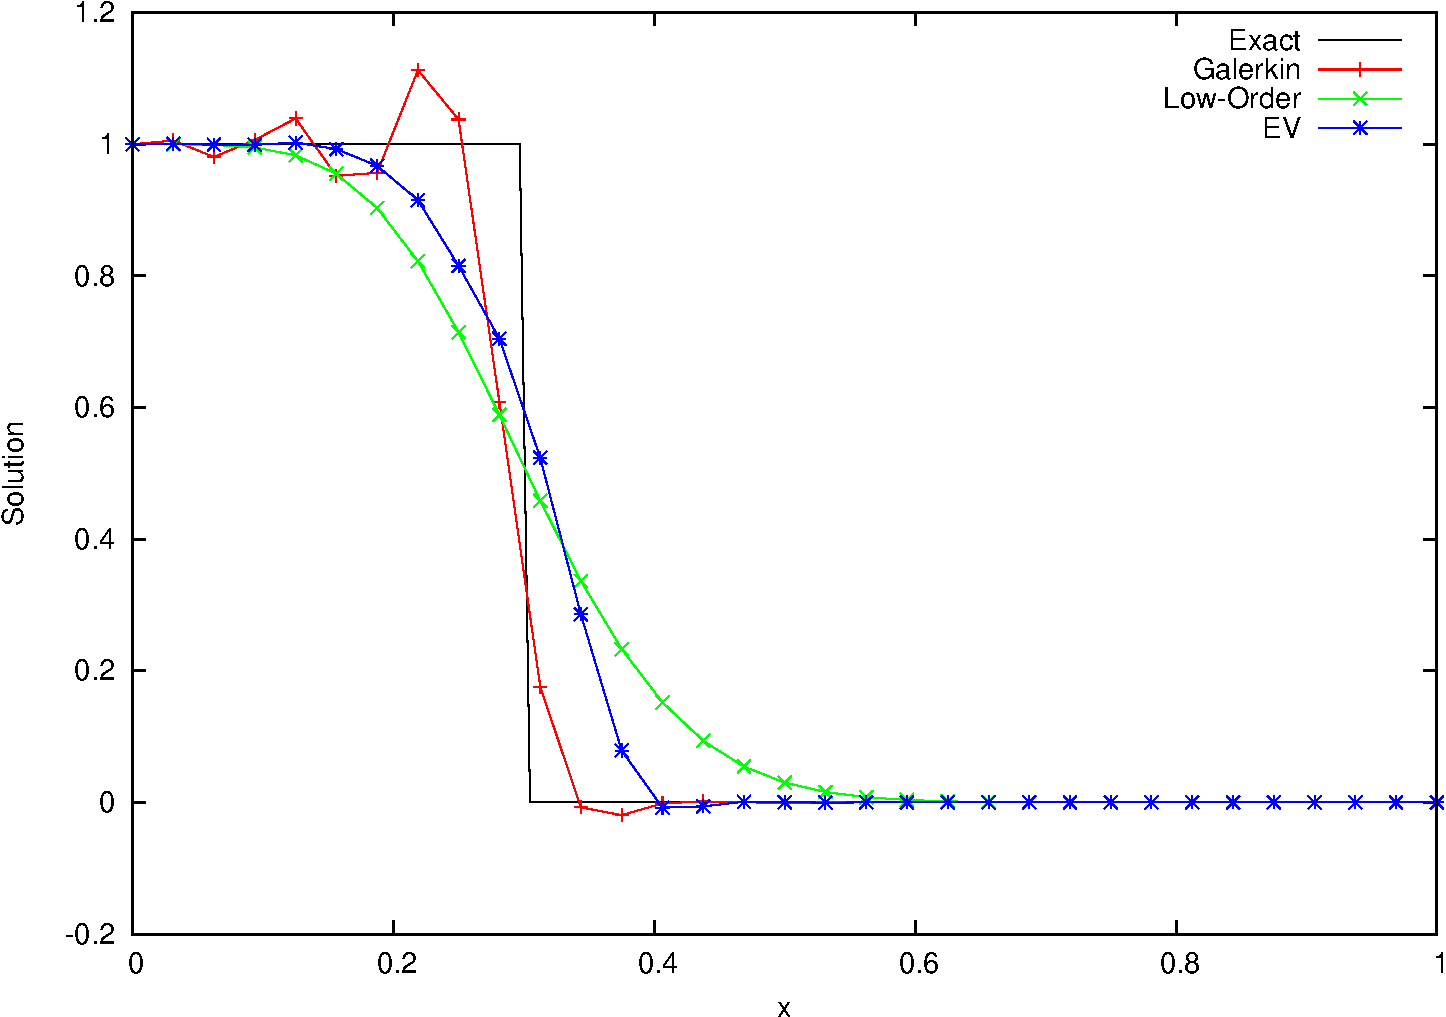
\includegraphics[width=0.85\textwidth]{./figures/advection_high_order.pdf}
\end{center}

\end{frame}
